\documentclass[11pt]{exam}

\usepackage{amsmath, amssymb, multicol}
\usepackage{graphicx}
\usepackage{textcomp}
\usepackage{chessboard}

\def\d{\displaystyle}
\def\b{\mathbf}
\def\R{\mathbf{R}}
\def\Z{\mathbf{Z}}
\def\st{~:~}
\def\bar{\overline}
\def\inv{^{-1}}

\def\v{circle (3pt)}
 \def\d{\displaystyle}
\def\?{\reflectbox{?}}
\def\b#1{\mathbf{#1}}
\def\f#1{\mathfrak #1}
\def\c#1{\mathcal #1}
\def\s#1{\mathscr #1}
\def\r#1{\mathrm{#1}}
\def\N{\mathbb N}
\def\Z{\mathbb Z}
\def\Q{\mathbb Q}
\def\R{\mathbb R}
\def\C{\mathbb C}
\def\F{\mathbb F}
\def\A{\mathbb A}
\def\X{\mathbb X}
\def\E{\mathbb E}
\def\O{\mathbb O}
\def\U{\mathcal U}
\def\pow{\mathcal P}
\def\inv{^{-1}}
\def\nrml{\triangleleft}
\def\st{:}
\def\~{\widetilde}
\def\rem{\mathcal R}
\def\sigalg{$\sigma$-algebra }
\def\Gal{\mbox{Gal}}
\def\iff{\leftrightarrow}
\def\Iff{\Leftrightarrow}
\def\land{\wedge}
\def\And{\bigwedge}
\def\AAnd{\d\bigwedge\mkern-18mu\bigwedge}
\def\Vee{\bigvee}
\def\VVee{\d\Vee\mkern-18mu\Vee}
\def\imp{\rightarrow}
\def\Imp{\Rightarrow}
\def\Fi{\Leftarrow}

%\def\={\equiv}
\def\var{\mbox{var}}
\def\mod{\mbox{Mod}}
\def\Th{\mbox{Th}}
\def\sat{\mbox{Sat}}
\def\con{\mbox{Con}}
\def\bmodels{=\joinrel\mathrel|}
\def\iffmodels{\bmodels\models}
\def\dbland{\bigwedge \!\!\bigwedge}
\def\dom{\mbox{dom}}
\def\rng{\mbox{range}}
\DeclareMathOperator{\wgt}{wgt}


\def\bar{\overline}


\newcommand{\vtx}[2]{node[fill,circle,inner sep=0pt, minimum size=4pt,label=#1:#2]{}}
\newcommand{\va}[1]{\vtx{above}{#1}}
\newcommand{\vb}[1]{\vtx{below}{#1}}
\newcommand{\vr}[1]{\vtx{right}{#1}}
\newcommand{\vl}[1]{\vtx{left}{#1}}
\renewcommand{\v}{\vtx{above}{}}

\def\circleA{(-.5,0) circle (1)}
\def\circleAlabel{(-1.5,.6) node[above]{$A$}}
\def\circleB{(.5,0) circle (1)}
\def\circleBlabel{(1.5,.6) node[above]{$B$}}
\def\circleC{(0,-1) circle (1)}
\def\circleClabel{(.5,-2) node[right]{$C$}}
\def\twosetbox{(-2,-1.4) rectangle (2,1.4)}
\def\threesetbox{(-2.5,-2.4) rectangle (2.5,1.4)}
\newcommand{\twoline}[2]{\begin{pmatrix}#1 \\ #2 \end{pmatrix}}



%\pointname{pts}
\pointsinmargin
\marginpointname{pts}
\addpoints
\pagestyle{head}
%\printanswers

\firstpageheader{Math 228}{\bf Counting Colorings with PIE}{Wednesday, November 14}


\begin{document}

%space for name
%\noindent {\large\bf Name:} \underline{\hspace{2.5in}}
%\vskip 1em

Recall, the \emph{chromatic polynomial} of a graph $G$, written $P(G,k)$ is a function in the variable $k$ that gives the number of proper $k$-colorings of $G$.

\begin{questions}
  \question Let's use PIE to find the chromatic polynomial of the path below.  You already know what the answer should be, but using PIE will give another way to compute this.
  \begin{center}
    {\footnotesize
      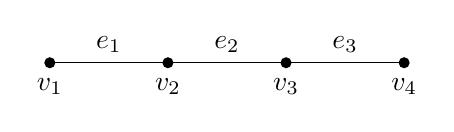
\begin{tikzpicture}[scale=1.5]
        \draw (0,0) \vb{$v_1$} -- (1,0) \vb{$v_2$} -- (2,0) \vb{$v_3$} -- (3,0) \vb{$v_4$};
        \draw (0,0) -- (1,0) node[midway, above]{$e_1$};
        \draw (1,0) -- (2,0) node[midway, above]{$e_2$};
        \draw (2,0) -- (3,0) node[midway, above]{$e_3$};
      \end{tikzpicture}
    }
  \end{center}
  \begin{parts}
    \part First, how many $k$-colorings are there, including all those that are not ``proper''?
    \vfill
    \part Now exclude those colorings that are not proper!  A coloring could not be proper because the vertices of $e_1$ are colored identically, or the vertices of $e_2$, or of $e_3$ or of $e_1$ and $e_2$, etc.  Make a table giving the number of colorings that have the vertices of each specified edge colored the same.

    \begin{center}
        \begin{tabular}{p{3.5cm}|p{1cm}|p{1cm}|p{1cm}|p{1.2cm}|p{1.2cm}|p{1.2cm}|p{2cm}}
          Edge(s) with same colored vertices & $e_1$ & $e_2$ & $e_3$ & $e_1$ \& $e_2$ & $e_1$ \& $e_3$ & $e_2$ \& $e_3$ & $e_1$, $e_2$, \& $e_3$ \\ \hline
          Number of $k$-colorings of $G$ & & & & & & &
        \end{tabular}
    \end{center}
\vskip 1em
    \part Use PIE to combine the numbers above to give the chromatic polynomial.
    \vfill
  \end{parts}



  \question Use PIE to find $P(C_5,k)$.  (The graph $C_5$ is the cycle on 5 vertices; label the edges $e_1, \ldots, e_5$ in counter-clockwise order.)
\vfill

\end{questions}


\end{document}
